\documentclass[10pt]{extarticle}

\usepackage[english]{babel}
\usepackage{graphicx}
\usepackage{framed}
\usepackage[normalem]{ulem}
\usepackage{indentfirst}
\usepackage{amsmath,amsthm,amssymb,amsfonts}
\usepackage{mathtools} % Wraparound amsmath. For fancy math typesetting
\usepackage[nointegrals]{wasysym} % nointegrals prevents wasysym from overwriting integral symbols from LaTeX and amsmath
\usepackage{bbm} % For extended bold and blackboard bold characters
\usepackage[italicdiff]{physics} % italicdiff causes derivatives to be rendered with italic d's instead of upright d's
\usepackage[T1]{fontenc}
\usepackage{xparse}
\usepackage{xstring}
% \usepackage{pifont} % For unusual symbols
% \usepackage{mathdots} % For unusual combinations of dots
\usepackage{wrapfig}
\usepackage{lmodern,mathrsfs}
\usepackage[inline,shortlabels]{enumitem}
\setlist{topsep=2pt,itemsep=2pt,parsep=0pt,partopsep=0pt}
\usepackage[table,dvipsnames]{xcolor}
\usepackage[utf8]{inputenc}
\usepackage{csquotes} % Must be loaded AFTER inputenc
\usepackage[a4paper,top=0.5in,bottom=0.2in,left=0.5in,right=0.5in,footskip=0.3in,includefoot]{geometry}
\usepackage[most]{tcolorbox}
\usepackage{tikz,tikz-3dplot,tikz-cd,tkz-tab,tkz-euclide,pgf,pgfplots}
\pgfplotsset{compat=newest}
% \usepackage{comment} % For commenting large blocks of text and math efficiently
% \usepackage{fancyvrb} % For custom verbatim environments
\usepackage{multicol}
\usepackage[bottom,multiple]{footmisc} % Ensures footnotes are at the bottom of the page, and separates footnotes by a comma if they are adjacent
\usepackage[backend=bibtex,style=numeric]{biblatex}
\renewcommand*{\finalnamedelim}{\addcomma\addspace} % Forces authors' names to be separated by comma, instead of "and"
\addbibresource{bibliography}
\usepackage[colorlinks,linkcolor=.,citecolor=blue,urlcolor=violet]{hyperref}
\usepackage[nameinlink]{cleveref} % nameinlink ensures that the entire element is clickable in the pdf, not just the number

\newcommand{\remind}[1]{\textcolor{red}{\textbf{#1}}} % To remind me of unfinished work to fix later
\newcommand{\hide}[1]{} % To hide large blocks of code without using % symbols

% Same as \href, but the text appears in typewriter font and in a custom color
\newcommand{\Href}[3][red!50!black]{\href{#2}{\textcolor{#1}{\texttt{#3}}}}

\newcommand{\ep}{\varepsilon}
\newcommand{\vp}{\varphi}
\newcommand{\lam}{\lambda}
\newcommand{\Lam}{\Lambda}
\DeclareDocumentCommand\ip{ l m }{\braces#1{\langle}{\rangle}{#2}} % Inner product ⟨x,y⟩ (but only one argument is taken, so \ip{x,y} renders as ⟨x,y⟩)
\DeclareDocumentCommand\floor{ l m }{\braces#1{\lfloor}{\rfloor}{#2}} % Floor function ⌊x⌋
\DeclareDocumentCommand\ceil{ l m }{\braces#1{\lceil}{\rceil}{#2}} % Ceiling function ⌈x⌉

% Shortcuts for blackboard bold letters, e.g. \A outputs \mathbb{A}
\def\do#1{\csdef{#1}{\mathbb{#1}}}
\docsvlist{A,B,C,D,E,F,G,I,J,K,M,N,Q,R,T,U,V,W,X,Y,Z}
% \H is already defined as a 1-argument command, it places a double acute accent (hungarumlaut) on a character, e.g. \H{o} yields ő
% \L is already defined as the uppercase Ł (L with stroke)
% \O is already defined as the uppercase Ø (O with stroke)
% \P is already defined as the pilcrow ¶ (paragraph mark)
% \S is already defined as the section sign §

% Shortcuts for calligraphic letters, e.g. \As outputs \mathcal{A}
\def\do#1{\csdef{#1s}{\mathcal{#1}}}
\docsvlist{A,B,C,D,E,F,G,H,I,J,K,L,M,N,O,P,Q,R,S,T,U,V,W,X,Y,Z}

% Shortcuts for letters with a bar on top, e.g. \Abar outputs \overline{A}
\def\do#1{\csdef{#1bar}{\overline{#1}}}
\docsvlist{a,b,c,d,e,f,g,i,j,k,l,m,n,o,p,q,r,s,t,u,v,w,x,y,z,A,B,C,D,E,F,G,H,I,J,K,L,M,N,O,P,Q,R,S,T,U,V,W,X,Y,Z}
% \hbar is already defined as the symbol ℏ (reduced Planck constant)

% Shortcuts for boldface letters, e.g. \Ab outputs \textbf{A}
\def\do#1{\csdef{#1b}{\textbf{#1}}}
\docsvlist{a,b,c,d,e,f,g,h,i,j,k,l,m,n,o,q,r,t,u,w,x,y,z,A,B,C,D,E,F,G,H,I,J,K,L,M,N,O,P,Q,R,S,T,U,V,W,X,Y,Z}
% \pb is already defined (by the physics package) as a 2-argument command, denoting the anticommutator or Poisson bracket, e.g. \pb{A,B} yields {A,B}
% \sb is already defined in the LaTeX kernel. This is a fundamental LaTeX command, DO NOT overwrite it!
% \vb is already defined (by the physics package) as a 1-argument command, for boldface text, e.g. \vb{A} yields \textbf{A}

% Shortcuts for letters with a tilde on top, e.g. \Atil outputs \widetilde{A}
\def\do#1{\csdef{#1til}{\widetilde{#1}}}
\docsvlist{a,b,c,d,e,f,g,h,i,j,k,l,m,n,o,p,q,r,s,t,u,v,w,x,y,z,A,B,C,D,E,F,G,H,I,J,K,L,M,N,O,P,Q,R,S,T,U,V,W,X,Y,Z}

\newcommand{\tm}{^{\mathsf{T}}}     % Transpose
\newcommand{\hm}{^{\mathsf{H}}}     % Conjugate transpose (Hermitian conjugate)
\newcommand{\itm}{^{-\mathsf{T}}}   % Inverse transpose
\newcommand{\ihm}{^{-\mathsf{H}}}   % Inverse conjugate transpose (Inverse Hermitian conjugate)
\newcommand{\ex}{\textbf{e}_x}
\newcommand{\ey}{\textbf{e}_y}
\newcommand{\ez}{\textbf{e}_z}
\newcommand{\Aint}{A^\circ}
\newcommand{\Bint}{B^\circ}
\newcommand{\limk}{\lim_{k\to\infty}}
\newcommand{\limm}{\lim_{m\to\infty}}
\newcommand{\limn}{\lim_{n\to\infty}}
\newcommand{\limx}[1][a]{\lim_{x\to#1}}
\newcommand{\limz}[1][{z_0}]{\lim_{z\to#1}}
\newcommand{\liminfm}{\liminf_{m\to\infty}}
\newcommand{\limsupm}{\limsup_{m\to\infty}}
\newcommand{\liminfn}{\liminf_{n\to\infty}}
\newcommand{\limsupn}{\limsup_{n\to\infty}}
\newcommand{\sumkn}{\sum_{k=1}^n}
\newcommand{\sumk}[1][1]{\sum_{k=#1}^\infty}
\newcommand{\summ}[1][1]{\sum_{m=#1}^\infty}
\newcommand{\sumn}[1][1]{\sum_{n=#1}^\infty}
\newcommand{\emp}{\varnothing}
\newcommand{\exc}{\backslash}
\newcommand{\sub}{\subseteq}
\newcommand{\sups}{\supseteq}
\newcommand{\capp}{\bigcap}
\newcommand{\cupp}{\bigcup}
\newcommand{\kupp}{\bigsqcup}
\newcommand{\cappkn}{\bigcap_{k=1}^n}
\newcommand{\cuppkn}{\bigcup_{k=1}^n}
\newcommand{\kuppkn}{\bigsqcup_{k=1}^n}
\newcommand{\cappk}[1][1]{\bigcap_{k=#1}^\infty}
\newcommand{\cuppk}[1][1]{\bigcup_{k=#1}^\infty}
\newcommand{\cappm}[1][1]{\bigcap_{m=#1}^\infty}
\newcommand{\cuppm}[1][1]{\bigcup_{m=#1}^\infty}
\newcommand{\cappn}[1][1]{\bigcap_{n=#1}^\infty}
\newcommand{\cuppn}[1][1]{\bigcup_{n=#1}^\infty}
\newcommand{\kuppk}[1][1]{\bigsqcup_{k=#1}^\infty}
\newcommand{\kuppm}[1][1]{\bigsqcup_{m=#1}^\infty}
\newcommand{\kuppn}[1][1]{\bigsqcup_{n=#1}^\infty}
\newcommand{\cappa}{\bigcap_{\alpha\in I}}
\newcommand{\cuppa}{\bigcup_{\alpha\in I}}
\newcommand{\kuppa}{\bigsqcup_{\alpha\in I}}
\newcommand{\dx}{\,dx}
\newcommand{\dy}{\,dy}
\newcommand{\dt}{\,dt}
\newcommand{\dmu}{\,d\mu}
\newcommand{\dnu}{\,d\nu}
\DeclareMathOperator{\glb}{\text{glb}}
\DeclareMathOperator{\lub}{\text{lub}}
\newcommand{\xh}{\widehat{x}}
\newcommand{\yh}{\widehat{y}}
\newcommand{\zh}{\widehat{z}}
\newcommand{\<}{\langle}
\renewcommand{\>}{\rangle}

% Shortcuts for inverse hyperbolic functions (and other operators with the same structure)
\def\do#1{\csdef{#1}{\trigbraces{\operatorname{#1}}}}
\docsvlist{
    asinh,acosh,atanh,acoth,asech,acsch,
    arsinh,arcosh,artanh,arcoth,arsech,arcsch,
    arcsinh,arccosh,arctanh,arccoth,arcsech,arccsch,
    sen,tg,cth,senh,tgh,ctgh,
    Re,Im,arg,Arg,im,ker
}

% \spn has to be defined separately as the syntax "spn" is different from the output "span"
% \span is already defined in the LaTeX kernel. This is a fundamental LaTeX command, DO NOT overwrite it!
\newcommand{\spn}{\trigbraces{\operatorname{span}}}

\makeatletter
% Redefining the commands \iff (given by LaTeX), \implies and \impliedby (given by amsmath)
% Math mode is automatically enforced, starred version makes the arrows shorter
\renewcommand{\impliedby}{\@ifstar{\ensuremath{\Longleftarrow}}{\ensuremath{\Leftarrow}}} % Corresponding Unicode character: U+21D0 ⇐
\renewcommand{\implies}{\@ifstar{\ensuremath{\Longrightarrow}}{\ensuremath{\Rightarrow}}} % Corresponding Unicode character: U+21D2 ⇒
\renewcommand{\iff}{\@ifstar{\ensuremath{\Longleftrightarrow}}{\ensuremath{\Leftrightarrow}}} % Corresponding Unicode character: U+21D4 ⇔
\makeatother

\newtheoremstyle{mystyle}{}{}{}{}{\sffamily\bfseries}{.}{ }{}
\makeatletter
\renewenvironment{proof}[1][\proofname] {\par\pushQED{\qed}{\normalfont\sffamily\bfseries\topsep6\p@\@plus6\p@\relax #1\@addpunct{.} }}{\popQED\endtrivlist\@endpefalse}
\makeatother
\renewcommand{\qedsymbol}{\coolqed{0.32}} % Implements the new QED symbol
\theoremstyle{mystyle}{\newtheorem*{remark}{Remark}}
\theoremstyle{mystyle}{\newtheorem*{remarks}{Remarks}}
\theoremstyle{mystyle}{\newtheorem*{example}{Example}}
\theoremstyle{mystyle}{\newtheorem*{examples}{Examples}}
\theoremstyle{definition}{\newtheorem*{exercise}{Exercise}}

% Warning environment
\newtheoremstyle{warn}{}{}{}{}{\normalfont}{}{ }{}
\theoremstyle{warn}
\newtheorem*{warning}{\warningsign{0.2}\relax}

% Symbol for the warning environment, designed to be easily scalable
\newcommand{\warningsign}[1]{
    \tikz[scale=#1,every node/.style={transform shape}]{
        \draw[-,line width={#1*0.8mm},red,fill=yellow,rounded corners={#1*2.5mm}] (0,0)--(1,{-sqrt(3)})--(-1,{-sqrt(3)})--cycle;
        \node at (0,-1) {\fontsize{48}{60}\selectfont\bfseries!};
}}

\newcommand{\coolqed}[1]{\includegraphics[width=#1cm]{sunglasses_emoji.png}} % QED symbol

% verbbox environment, for showing verbatim text next to code output (for package documentation and user learning purposes)
\NewTCBListing{verbbox}{ !O{} }{boxrule=1pt,sidebyside,skin=bicolor,colback=gray!10,colbacklower=white,valign=center,top=2pt,bottom=2pt,left=2pt,right=2pt,#1} % Last argument allows more tcolorbox options to be added

\NewDocumentCommand{\solidball}{ s O{} m O{white} m }{
\tikz[scale=#5,every node/.style={transform shape}]{
    \shade[ball color=#3] (0,0) circle (0.5); %solid ball with no label
    \IfBooleanF{#1}{
        \clip (0,0) circle (0.25);
        \shade[ball color=#4] (0,0) circle (0.5);
    }
    \node[font=\sffamily\bfseries\selectfont] at (0,0) {#2}; % Label
}
}

\NewDocumentCommand{\stripedball}{ s O{} m O{white} m }{
\tikz[scale=#5,every node/.style={transform shape}]{
    \shade[ball color=#4] (0,0) circle (0.5);
    \clip (-0.5,-0.35) rectangle (0.5,0.35);
    \shade[ball color=#3] (0,0) circle (0.5);
    \IfBooleanF{#1}{
        \clip (0,0) circle (0.25);
        \shade[ball color=#4] (0,0) circle (0.5);
    }
    \node[font=\sffamily\bfseries\selectfont] at (0,0) {#2}; % Label
}
}

% Official colors for Aramith Tournament pool balls
% Colors taken from https://www.aramith.com/story-behind-aramith-tournament-black-colours
\definecolor{aramith_color_0}{HTML}{FFFFDF} % Cue ball and secondary color for all balls
\definecolor{aramith_color_1}{HTML}{FFD501} % 1 and 9
\definecolor{aramith_color_2}{HTML}{013CB1} % 2 and 10
\definecolor{aramith_color_3}{HTML}{E71C01} % 3 and 11
\definecolor{aramith_color_4}{HTML}{4F029C} % 4 and 12
\definecolor{aramith_color_5}{HTML}{FA4D00} % 5 and 13
\definecolor{aramith_color_6}{HTML}{0E5D01} % 6 and 14
\definecolor{aramith_color_7}{HTML}{6D071A} % 7 and 15
\definecolor{aramith_color_8}{HTML}{000000} % 8 (black)


\makeatletter
% Adapted from https://tex.stackexchange.com/a/61600
\csdef{aramith_pool_ball@0}#1{\solidball*{aramith_color_0}{#1}}                         % Cue ball
\csdef{aramith_pool_ball@1}#1{\solidball[1]{aramith_color_1}[aramith_color_0]{#1}}      % Ball 1
\csdef{aramith_pool_ball@2}#1{\solidball[2]{aramith_color_2}[aramith_color_0]{#1}}      % Ball 2
\csdef{aramith_pool_ball@3}#1{\solidball[3]{aramith_color_3}[aramith_color_0]{#1}}      % Ball 3
\csdef{aramith_pool_ball@4}#1{\solidball[4]{aramith_color_4}[aramith_color_0]{#1}}      % Ball 4
\csdef{aramith_pool_ball@5}#1{\solidball[5]{aramith_color_5}[aramith_color_0]{#1}}      % Ball 5
\csdef{aramith_pool_ball@6}#1{\solidball[6]{aramith_color_6}[aramith_color_0]{#1}}      % Ball 6
\csdef{aramith_pool_ball@7}#1{\solidball[7]{aramith_color_7}[aramith_color_0]{#1}}      % Ball 7
\csdef{aramith_pool_ball@8}#1{\solidball[8]{aramith_color_8}[aramith_color_0]{#1}}      % Ball 8 (black)
\csdef{aramith_pool_ball@9}#1{\stripedball[9]{aramith_color_1}[aramith_color_0]{#1}}    % Ball 9
\csdef{aramith_pool_ball@10}#1{\stripedball[10]{aramith_color_2}[aramith_color_0]{#1}}  % Ball 10
\csdef{aramith_pool_ball@11}#1{\stripedball[11]{aramith_color_3}[aramith_color_0]{#1}}  % Ball 11
\csdef{aramith_pool_ball@12}#1{\stripedball[12]{aramith_color_4}[aramith_color_0]{#1}}  % Ball 12
\csdef{aramith_pool_ball@13}#1{\stripedball[13]{aramith_color_5}[aramith_color_0]{#1}}  % Ball 13
\csdef{aramith_pool_ball@14}#1{\stripedball[14]{aramith_color_6}[aramith_color_0]{#1}}  % Ball 14
\csdef{aramith_pool_ball@15}#1{\stripedball[15]{aramith_color_7}[aramith_color_0]{#1}}  % Ball 15
\NewDocumentCommand{\poolball}{ o m m }{
    \pgfmathparse{Mod(#2,16)} % Argument #2 mod 16  as a floating-point number, e.g. 4.0
    \pgfmathtruncatemacro{\argumentmodulosixteen}{\pgfmathresult} % Convert to integer, e.g. 4.0 to 4
    \ifnum\argumentmodulosixteen=0
        \solidball*{aramith_color_0}{#3}
    \else
        \ifnum\argumentmodulosixteen<9
            \solidball[\IfNoValueTF{#1}{#2}{#1}]{aramith_color_\argumentmodulosixteen}[aramith_color_0]{#3} % Solid ball of the appropriate color, and the appropriate number (if the optional argument is not specified), otherwise the optional argument
        \else
            \pgfmathparse{\argumentmodulosixteen-8} % Argument #2 mod 8  as a floating-point number, e.g. 3.0 (this will only be computed if #2≥9)
            \pgfmathtruncatemacro{\argumentmoduloeight}{\pgfmathresult} % Convert to integer, e.g. 3.0 to 3
            \stripedball[\IfNoValueTF{#1}{#2}{#1}]{aramith_color_\argumentmoduloeight}[aramith_color_0]{#3} % Striped ball of the appropriate color, and the appropriate number (if the optional argument is not specified), otherwise the optional argument
        \fi
    \fi}
\makeatother

\makeatletter
% \fsize stores the current font size but is expandable (and can be called later without using \makeatletter and \makeatother)
\def\fsize{\dimexpr\f@size pt\relax}
\makeatother

\makeatletter
% Adapted from https://tex.stackexchange.com/a/19700
\def\my@vector #1,#2\@eolst{
    \ifx\relax#2\relax
        #1
    \else
        #1\my@delim
        \my@vector #2\@eolst
    \fi}
\newcommand\vcstring[2][\\]{% Converts comma-separated string to #1-separated string
    \def\my@delim{#1}
        \my@vector #2,\relax\noexpand\@eolst}
\newcommand\cvc[2][p]{% Converts comma-separated string to column vector, optional argument defines matrix brackets
    \def\my@delim{\\}
        \begin{#1matrix} % Empty argument also possible
            \my@vector #2,\relax\noexpand\@eolst
        \end{#1matrix}}
\newcommand\rvc[2][p]{% Converts comma-separated string to row vector, optional argument defines matrix brackets
    \def\my@delim{&}
        \begin{#1matrix} % Empty argument also possible
            \my@vector #2,\relax\noexpand\@eolst
        \end{#1matrix}}
% Matrix environment with variable number of arguments. Adapted from https://davidyat.es/2016/07/27/writing-a-latex-macro-that-takes-a-variable-number-of-arguments/
\newcommand{\mat}[2][p]{
    \def\matrixenvironment{#1matrix} % Specifying the matrix brackets, this has to be done beforehand as '#1' changes under \passtonextarg
    \def\my@delim{&}
        \begin{\matrixenvironment} % Begin matrix environment
            \my@vector #2,\relax\noexpand\@eolst
            \@ifnextchar\bgroup{\passtonextarg}{\end{\matrixenvironment}}% % Pass to next argument (if any), otherwise end matrix environment
}
\newcommand{\passtonextarg}[1]{\\ \my@vector #1,\relax\noexpand\@eolst
    \@ifnextchar\bgroup{\passtonextarg}{\end{\matrixenvironment}}% Passing to next argument
}
\makeatother

\definecolor{tcol_DEF}{HTML}{E40125} % Color for Definition
\definecolor{tcol_PRP}{HTML}{EB8407} % Color for Proposition
\definecolor{tcol_LEM}{HTML}{05C4D9} % Color for Lemma
\definecolor{tcol_THM}{HTML}{1346E4} % Color for Theorem
\definecolor{tcol_COR}{HTML}{7904C2} % Color for Corollary
\definecolor{tcol_REM}{HTML}{18B640} % Color for Remark
\definecolor{tcol_PRF}{HTML}{5A76B2} % Color for Proof
\definecolor{tcol_EXA}{HTML}{21340A} % Color for Example

\tcbset{
tbox_DEF_style/.style={enhanced jigsaw,
    colback=tcol_DEF!10,colframe=tcol_DEF!80!black,,
    fonttitle=\sffamily\bfseries,
    separator sign=.,label separator={},
    sharp corners,top=2pt,bottom=2pt,left=2pt,right=2pt,
    before skip=10pt,after skip=10pt,breakable
},
tbox_PRP_style/.style={enhanced jigsaw,
    colback=tcol_PRP!10,colframe=tcol_PRP!80!black,
    fonttitle=\sffamily\bfseries,
    attach boxed title to top left={yshift=-\tcboxedtitleheight},
    boxed title style={
        boxrule=0pt,boxsep=2.5pt,
        colback=tcol_PRP!80!black,colframe=tcol_PRP!80!black,
        sharp corners=uphill
    },
    separator sign=.,label separator={},
    top=\tcboxedtitleheight,bottom=2pt,left=2pt,right=2pt,
    before skip=10pt,after skip=10pt,drop fuzzy shadow,breakable
},
tbox_THM_style/.style={enhanced jigsaw,
    colback=tcol_THM!10,colframe=tcol_THM!80!black,
    fonttitle=\sffamily\bfseries,coltitle=black,
    attach boxed title to top left={xshift=10pt,yshift=-\tcboxedtitleheight/2},
    boxed title style={
        colback=tcol_THM!10,colframe=tcol_THM!80!black,height=16pt,bean arc
    },
    separator sign=.,label separator={},
    sharp corners,top=6pt,bottom=2pt,left=2pt,right=2pt,
    before skip=10pt,after skip=10pt,breakable
},
tbox_LEM_style/.style={enhanced jigsaw,
    colback=tcol_LEM!10,colframe=tcol_LEM!80!black,
    boxrule=0pt,
    fonttitle=\sffamily\bfseries,
    attach boxed title to top left={yshift=-\tcboxedtitleheight},
    boxed title style={
        boxrule=0pt,boxsep=2pt,
        colback=tcol_LEM!80!black,colframe=tcol_LEM!80!black,
        interior code={\fill[tcol_LEM!80!black] (interior.north west)--(interior.south west)--([xshift=-2mm]interior.south east)--([xshift=2mm]interior.north east)--cycle;
    }},
    separator sign=.,label separator={},
    frame hidden,borderline north={1pt}{0pt}{tcol_LEM!80!black},
    before upper={\hspace{\tcboxedtitlewidth}},
    sharp corners,top=2pt,bottom=2pt,left=5pt,right=5pt,
    before skip=10pt,after skip=10pt,breakable
},
tbox_COR_style/.style={enhanced jigsaw,
    colback=tcol_COR!10,colframe=tcol_COR!80!black,
    boxrule=0pt,
    fonttitle=\sffamily\bfseries,coltitle=black,
    separator sign={},label separator={},
    description font=\normalfont\sffamily,
    description delimiters={(}{)},
    attach title to upper,after title={.\ },
    frame hidden,borderline west={2pt}{0pt}{tcol_COR},
    sharp corners,top=2pt,bottom=2pt,left=5pt,right=5pt,
    before skip=10pt,after skip=10pt,breakable
},
}

\newtcbtheorem[number within=section,
    crefname={\color{tcol_DEF!50!black} definition}{\color{tcol_DEF!50!black} definitions},
    Crefname={\color{tcol_DEF!50!black} Definition}{\color{tcol_DEF!50!black} Definitions}
    ]{definition}{Definition}{tbox_DEF_style}{}
\newtcbtheorem[use counter from=definition,
    crefname={\color{tcol_PRP!50!black} proposition}{\color{tcol_PRP!50!black} propositions},
    Crefname={\color{tcol_PRP!50!black} Proposition}{\color{tcol_PRP!50!black} Propositions}
    ]{proposition}{Proposition}{tbox_PRP_style}{}
\newtcbtheorem[use counter from=definition,
    crefname={\color{tcol_THM!50!black} theorem}{\color{tcol_THM!50!black} theorems},
    Crefname={\color{tcol_THM!50!black} Theorem}{\color{tcol_THM!50!black} Theorems}
    ]{theorem}{Theorem}{tbox_THM_style}{}
\newtcbtheorem[use counter from=definition,
    crefname={\color{tcol_LEM!50!black} lemma}{\color{tcol_LEM!50!black} lemmas},
    Crefname={\color{tcol_LEM!50!black} Lemma}{\color{tcol_LEM!50!black} Lemmas}
    ]{lemma}{Lemma}{tbox_LEM_style}{}
\newtcbtheorem[use counter from=definition,
    crefname={\color{tcol_COR!50!black} corollary}{\color{tcol_COR!50!black} corollaries},
    Crefname={\color{tcol_COR!50!black} Corollary}{\color{tcol_COR!50!black} Corollaries}
    ]{corollary}{Corollary}{tbox_COR_style}{}

\makeatletter
\@namedef{tcolorboxshape@filingbox@ul}#1#2#3{
    (frame.south west)--(title.north west)--([xshift=-\dimexpr#1\relax]title.north east) to[out=0,in=180] ([xshift=\dimexpr#2\relax,yshift=\dimexpr#3\relax]title.south east)--(frame.north east)--(frame.south east)--cycle
}
\@namedef{tcolorboxshape@filingbox@uc}#1#2#3{
    (frame.south west)--(frame.north west)--([xshift=-\dimexpr#2\relax,yshift=\dimexpr#3\relax]title.south west) to[out=0,in=180] ([xshift=\dimexpr#1\relax]title.north west)--([xshift=-\dimexpr#1\relax]title.north east) to[out=0,in=180] ([xshift=\dimexpr#2\relax,yshift=\dimexpr#3\relax]title.south east)--(frame.north east)--(frame.south east)--cycle
}
\@namedef{tcolorboxshape@filingbox@ur}#1#2#3{
    (frame.south east)--(title.north east)--([xshift=\dimexpr#1\relax]title.north west) to[out=180,in=0] ([xshift=-\dimexpr#2\relax,yshift=\dimexpr#3\relax]title.south west)--(frame.north west)--(frame.south west)--cycle
}
\@namedef{tcolorboxshape@filingbox@dl}#1#2#3{
    (frame.north west)--(title.south west)--([xshift=-\dimexpr#1\relax]title.south east) to[out=0,in=180] ([xshift=\dimexpr#2\relax,yshift=-\dimexpr#3\relax]title.north east)--(frame.south east)--(frame.north east)--cycle
}
\@namedef{tcolorboxshape@filingbox@dc}#1#2#3{
    (frame.north west)--(frame.south west)--([xshift=-\dimexpr#2\relax,yshift=-\dimexpr#3\relax]title.north west) to[out=0,in=180] ([xshift=\dimexpr#1\relax]title.south west)--([xshift=-\dimexpr#1\relax]title.south east) to[out=0,in=180] ([xshift=\dimexpr#2\relax,yshift=-\dimexpr#3\relax]title.north east)--(frame.south east)--(frame.north east)--cycle
}
\@namedef{tcolorboxshape@filingbox@dr}#1#2#3{
    (frame.north east)--(title.south east)--([xshift=\dimexpr#1\relax]title.south west) to[out=180,in=0] ([xshift=-\dimexpr#2\relax,yshift=-\dimexpr#3\relax]title.north west)--(frame.south west)--(frame.north west)--cycle
}
\@namedef{tcolorboxshape@railingbox@ul}#1#2#3{
    (frame.south west)--(title.north west)--([xshift=-\dimexpr#1\relax]title.north east)--([xshift=\dimexpr#2\relax,yshift=\dimexpr#3\relax]title.south east)--(frame.north east)--(frame.south east)--cycle
}
\@namedef{tcolorboxshape@railingbox@uc}#1#2#3{
    (frame.south west)--(frame.north west)--([xshift=-\dimexpr#2\relax,yshift=\dimexpr#3\relax]title.south west)--([xshift=\dimexpr#1\relax]title.north west)--([xshift=-\dimexpr#1\relax]title.north east)--([xshift=\dimexpr#2\relax,yshift=\dimexpr#3\relax]title.south east)--(frame.north east)--(frame.south east)--cycle
}
\@namedef{tcolorboxshape@railingbox@ur}#1#2#3{
    (frame.south east)--(title.north east)--([xshift=\dimexpr#1\relax]title.north west)--([xshift=-\dimexpr#2\relax,yshift=\dimexpr#3\relax]title.south west)--(frame.north west)--(frame.south west)--cycle
}
\@namedef{tcolorboxshape@railingbox@dl}#1#2#3{
    (frame.north west)--(title.south west)--([xshift=-\dimexpr#1\relax]title.south east)--([xshift=\dimexpr#2\relax,yshift=-\dimexpr#3\relax]title.north east)--(frame.south east)--(frame.north east)--cycle
}
\@namedef{tcolorboxshape@railingbox@dc}#1#2#3{
    (frame.north west)--(frame.south west)--([xshift=-\dimexpr#2\relax,yshift=-\dimexpr#3\relax]title.north west)--([xshift=\dimexpr#1\relax]title.south west)--([xshift=-\dimexpr#1\relax]title.south east)--([xshift=\dimexpr#2\relax,yshift=-\dimexpr#3\relax]title.north east)--(frame.south east)--(frame.north east)--cycle
}
\@namedef{tcolorboxshape@railingbox@dr}#1#2#3{
    (frame.north east)--(title.south east)--([xshift=\dimexpr#1\relax]title.south west)--([xshift=-\dimexpr#2\relax,yshift=-\dimexpr#3\relax]title.north west)--(frame.south west)--(frame.north west)--cycle
}
\newcommand{\TColorBoxShape}[2]{\expandafter\ifx\csname tcolorboxshape@#1@#2\endcsname\relax
\expandafter\@gobble\else
\csname tcolorboxshape@#1@#2\expandafter\endcsname
\fi}
\makeatother

\tcbset{ % Styles for filingbox, railingbox and flagbox environments
% Adapted from https://tex.stackexchange.com/questions/587912/tcolorbox-custom-title-box-style
filingstyle/ul/.style 2 args={
    attach boxed title to top left={yshift=-2mm},
    boxed title style={empty,top=0mm,bottom=1mm,left=1mm,right=0mm},
    interior code={
        \path[fill=#1,rounded corners] \TColorBoxShape{filingbox}{ul}{9pt}{18pt}{6pt};
    },
    frame code={
        \path[draw=#2,line width=0.5mm,rounded corners] \TColorBoxShape{filingbox}{ul}{9pt}{18pt}{6pt};
    }},
filingstyle/uc/.style 2 args={
    attach boxed title to top center={yshift=-2mm},
    boxed title style={empty,top=0mm,bottom=1mm,left=0mm,right=0mm},
    interior code={
        \path[fill=#1,rounded corners] \TColorBoxShape{filingbox}{uc}{9pt}{18pt}{6pt};
    },
    frame code={
        \path[draw=#2,line width=0.5mm,rounded corners] \TColorBoxShape{filingbox}{uc}{9pt}{18pt}{6pt};
    }},
filingstyle/ur/.style 2 args={
    attach boxed title to top right={yshift=-2mm},
    boxed title style={empty,top=0mm,bottom=1mm,left=0mm,right=1mm},
    interior code={
        \path[fill=#1,rounded corners] \TColorBoxShape{filingbox}{ur}{9pt}{18pt}{6pt};
    },
    frame code={
        \path[draw=#2,line width=0.5mm,rounded corners] \TColorBoxShape{filingbox}{ur}{9pt}{18pt}{6pt};
    }},
filingstyle/dl/.style 2 args={
    attach boxed title to bottom left={yshift=2mm},
    boxed title style={empty,top=1mm,bottom=0mm,left=1mm,right=0mm},
    interior code={
        \path[fill=#1,rounded corners] \TColorBoxShape{filingbox}{dl}{9pt}{18pt}{6pt};
    },
    frame code={
        \path[draw=#2,line width=0.5mm,rounded corners] \TColorBoxShape{filingbox}{dl}{9pt}{18pt}{6pt};
    }},
filingstyle/dc/.style 2 args={
    attach boxed title to bottom center={yshift=2mm},
    boxed title style={empty,top=1mm,bottom=0mm,left=0mm,right=0mm},
    interior code={
        \path[fill=#1,rounded corners] \TColorBoxShape{filingbox}{dc}{9pt}{18pt}{6pt};
    },
    frame code={
        \path[draw=#2,line width=0.5mm,rounded corners] \TColorBoxShape{filingbox}{dc}{9pt}{18pt}{6pt};
    }},
filingstyle/dr/.style 2 args={
    attach boxed title to bottom right={yshift=2mm},
    boxed title style={empty,top=1mm,bottom=0mm,left=0mm,right=1mm},
    interior code={
        \path[fill=#1,rounded corners] \TColorBoxShape{filingbox}{dr}{9pt}{18pt}{6pt};
    },
    frame code={
        \path[draw=#2,line width=0.5mm,rounded corners] \TColorBoxShape{filingbox}{dr}{9pt}{18pt}{6pt};
    }},
railingstyle/ul/.style 2 args={
    attach boxed title to top left={yshift=-2mm},
    boxed title style={empty,top=0mm,bottom=1mm,left=1mm,right=0mm},
    interior code={
        \path[fill=#1] \TColorBoxShape{railingbox}{ul}{3pt}{12pt}{6pt};
    },
    frame code={
        \path[draw=#2,line width=0.5mm] \TColorBoxShape{railingbox}{ul}{3pt}{12pt}{6pt};
    }},
railingstyle/uc/.style 2 args={
    attach boxed title to top center={yshift=-2mm},
    boxed title style={empty,top=0mm,bottom=1mm,left=0mm,right=0mm},
    interior code={
        \path[fill=#1] \TColorBoxShape{railingbox}{uc}{3pt}{12pt}{6pt};
    },
    frame code={
        \path[draw=#2,line width=0.5mm] \TColorBoxShape{railingbox}{uc}{3pt}{12pt}{6pt};
    }},
railingstyle/ur/.style 2 args={
    attach boxed title to top right={yshift=-2mm},
    boxed title style={empty,top=0mm,bottom=1mm,left=0mm,right=1mm},
    interior code={
        \path[fill=#1] \TColorBoxShape{railingbox}{ur}{3pt}{12pt}{6pt};
    },
    frame code={
        \path[draw=#2,line width=0.5mm] \TColorBoxShape{railingbox}{ur}{3pt}{12pt}{6pt};
    }},
railingstyle/dl/.style 2 args={
    attach boxed title to bottom left={yshift=2mm},
    boxed title style={empty,top=1mm,bottom=0mm,left=1mm,right=0mm},
    interior code={
        \path[fill=#1] \TColorBoxShape{railingbox}{dl}{3pt}{12pt}{6pt};
    },
    frame code={
        \path[draw=#2,line width=0.5mm] \TColorBoxShape{railingbox}{dl}{3pt}{12pt}{6pt};
    }},
railingstyle/dc/.style 2 args={
    attach boxed title to bottom center={yshift=2mm},
    boxed title style={empty,top=1mm,bottom=0mm,left=0mm,right=0mm},
    interior code={
        \path[fill=#1] \TColorBoxShape{railingbox}{dc}{3pt}{12pt}{6pt};
    },
    frame code={
        \path[draw=#2,line width=0.5mm] \TColorBoxShape{railingbox}{dc}{3pt}{12pt}{6pt};
    }},
railingstyle/dr/.style 2 args={
    attach boxed title to bottom right={yshift=2mm},
    boxed title style={empty,top=1mm,bottom=0mm,left=0mm,right=1mm},
    interior code={
        \path[fill=#1] \TColorBoxShape{railingbox}{dr}{3pt}{12pt}{6pt};
    },
    frame code={
        \path[draw=#2,line width=0.5mm] \TColorBoxShape{railingbox}{dr}{3pt}{12pt}{6pt};
    }},
flagstyle/ul/.style 2 args={
    interior hidden,frame hidden,colbacktitle=#1,
    borderline west={1pt}{0pt}{#2},
    attach boxed title to top left={yshift=-8pt,yshifttext=-8pt},
    boxed title style={boxsep=3pt,boxrule=1pt,colframe=#2,sharp corners,left=4pt,right=4pt},
    bottom=0mm
    },
flagstyle/ur/.style 2 args={
    interior hidden,frame hidden,colbacktitle=#1,
    borderline east={1pt}{0pt}{#2},
    attach boxed title to top right={yshift=-8pt,yshifttext=-8pt},
    boxed title style={boxsep=3pt,boxrule=1pt,colframe=#2,sharp corners,left=4pt,right=4pt},
    bottom=0mm
    },
flagstyle/dl/.style 2 args={
    interior hidden,frame hidden,colbacktitle=#1,
    borderline west={1pt}{0pt}{#2},
    attach boxed title to bottom left={yshift=8pt,yshifttext=8pt},
    boxed title style={boxsep=3pt,boxrule=1pt,colframe=#2,sharp corners,left=4pt,right=4pt},
    top=0mm
    },
flagstyle/dr/.style 2 args={
    interior hidden,frame hidden,colbacktitle=#1,
    borderline east={1pt}{0pt}{#2},
    attach boxed title to bottom right={yshift=8pt,yshifttext=8pt},
    boxed title style={boxsep=3pt,boxrule=1pt,colframe=#2,sharp corners,left=4pt,right=4pt},
    top=0mm
    }
}

% Box in the shape of a filing divider, position of tab can be ul (up left), uc (up center), ur (up right), dl (down left), dc (down center) or dr (down right). Default is ul (upper left)
\NewTColorBox{filingbox}{ D(){ul} O{black} m O{} }{enhanced,
    top=1mm,bottom=1mm,left=1mm,right=1mm,
    title={#3},
    fonttitle=\sffamily\bfseries,
    coltitle=black,
    filingstyle/#1={#2!10}{#2},
    #4
}

% Box in the shape of a railing bar, position of tab can be ul (up left), uc (up center), ur (up right), dl (down left), dc (down center) or dr (down right). Default is ul (upper left)
\NewTColorBox{railingbox}{ D(){ul} O{black} m O{} }{enhanced,
    top=1mm,bottom=1mm,left=1mm,right=1mm,
    title={#3},
    fonttitle=\sffamily\bfseries,
    coltitle=black,
    railingstyle/#1={#2!10}{#2},
    #4
}

% Box in the shape of a flag, position of tab can be ul (up left), ur (up right), dl (down left) or dr (down right). Default is ul (upper left)
\NewTColorBox{flagbox}{ D(){ul} O{black} m O{} }{enhanced,breakable,
    top=1mm,bottom=1mm,left=1mm,right=1mm,
    title={#3},
    fonttitle=\sffamily\bfseries,
    coltitle=black,
    flagstyle/#1={#2!10}{#2},
    #4
}

\makeatletter
\newcommand*{\CreateSmartLargeOperator}[2]{
% Adapted from https://tex.stackexchange.com/questions/61598/new-command-with-cases-conditionals-if-thens/61600
    % Plain operator (no customization)
    \csdef{LargeOperator@#1@}{\csdef{LargeOperator@#1@Symbol}{\csuse{#1}}}
    % Operator with limits above and below symbol
    \csdef{LargeOperator@#1@l}{\csdef{LargeOperator@#1@Symbol}{\csuse{#1}\limits}}
    % Operato with limits beside symbol
    \csdef{LargeOperator@#1@n}{\csdef{LargeOperator@#1@Symbol}{\csuse{#1}\nolimits}}
    % Inline style operator
    \csdef{LargeOperator@#1@i}{\csdef{LargeOperator@#1@Symbol}{\textstyle\csuse{#1}}}
    % Display style operator
    \csdef{LargeOperator@#1@d}{\csdef{LargeOperator@#1@Symbol}{\displaystyle\csuse{#1}}}
    % Inline style operator with limits above and below symbol
    \csdef{LargeOperator@#1@il}{\csdef{LargeOperator@#1@Symbol}{\textstyle\csuse{#1}\limits}}
    % Inline style operator with limits beside symbol
    \csdef{LargeOperator@#1@in}{\csdef{LargeOperator@#1@Symbol}{\textstyle\csuse{#1}\nolimits}}
    % Display style operator with limits above and below symbol
    \csdef{LargeOperator@#1@dl}{\csdef{LargeOperator@#1@Symbol}{\displaystyle\csuse{#1}\limits}}
    % Display style operator with limits beside symbol
    \csdef{LargeOperator@#1@dn}{\csdef{LargeOperator@#1@Symbol}{\displaystyle\csuse{#1}\nolimits}}

% NOTE: In the command below, ##1 denotes the operator. It is NOT to be used as an argument!
\def\LargeOperatorSpecs@i##1,##2,##3,##4,##5,##6,##7\@nil{
% If no arguments, operate over n from 1 to infinity
    \ifx$##2$\csuse{LargeOperator@##1@Symbol}_{n=1}^{\infty}\else
    % If one argument, operate over n from ##2 to infinity
        \ifx$##3$\csuse{LargeOperator@##1@Symbol}_{n=##2}^{\infty}\else
        % If two arguments, operate over n from ##2 to ##3
            \ifx$##4$\csuse{LargeOperator@##1@Symbol}_{n=##2}^{##3}\else
            % If three arguments, operate over ##2 from ##3 to ##4
                \ifx$##5$\csuse{LargeOperator@##1@Symbol}_{##2=##3}^{##4}\else
                % If four arguments, operate over ##2 and ##3 from ##4 to ##5
                    \ifx$##6$\csuse{LargeOperator@##1@Symbol}_{##2,##3=##4}^{##5}\else
                    % If five arguments, operate over ##2, ##3 and ##4 from ##5 to ##6
                        \csuse{LargeOperator@##1@Symbol}_{##2,##3,##4=##5}^{##6}
                    \fi
                \fi
            \fi
        \fi
    \fi
}

% Flexible "smart" large operator macro with comma-separated arguments and optional argument for formatting. Default is over n from 1 to infinity. Adapted from https://tex.stackexchange.com/a/15722
\expandafter\DeclareDocumentCommand\csname#2\endcsname{ O{} m }{ % New operator macro
\bgroup % Group created to keep operator style (e.g. \limits) local
    \expandafter\ifx\csname LargeOperator@#1@##1\endcsname\relax
    \expandafter\@gobble\else
    \csname LargeOperator@#1@##1\expandafter\endcsname
    \fi
    \expandafter\LargeOperatorSpecs@i#1,##2,,,,,\@nil% % #1 stands in for the first "argument" of \LargeOperatorSpecs@i (the operator), the actual arguments are from ##2 onward
\egroup}
}
\makeatother

% Create the smart large operator #2 based on the large operator #1. For example, \CreateSmartLargeOperator{sum}{Sum} will define \Sum as the smart large operator based on \sum
% Equivalent Unicode characters are given here (but they are NOT the same as the operators)
\CreateSmartLargeOperator{sum}{Sum}             % Large: U+2211 ∑ (no small version)
\CreateSmartLargeOperator{prod}{Prod}           % Small: U+2293 ⊓, Large: U+220F ∏
\CreateSmartLargeOperator{coprod}{Coprod}       % Small: U+2294 ⊔, Large: U+2210 ∐
\CreateSmartLargeOperator{bigcap}{Capp}         % Small: U+2229 ∩, Large: U+22C2 ⋂
\CreateSmartLargeOperator{bigcup}{Cupp}         % Small: U+222A ∪, Large: U+22C3 ⋃
\CreateSmartLargeOperator{bigsqcup}{Kupp}       % Small: U+2294 ⊔, Large: U+2210 ∐
\CreateSmartLargeOperator{bigodot}{Odot}        % Small: U+2299 ⊙ (no large version)
\CreateSmartLargeOperator{bigoplus}{Oplus}      % Small: U+2295 ⊕ (no large version)
\CreateSmartLargeOperator{bigotimes}{Otimes}    % Small: U+2297 ⊗ (no large version)
\CreateSmartLargeOperator{biguplus}{Uplus}      % Small: U+228E ⊎ (no large version)
\CreateSmartLargeOperator{bigwedge}{Wedge}      % Small: U+2227 ∧, Large: U+22C0 ⋀
\CreateSmartLargeOperator{bigvee}{Vee}          % Small: U+2228 ∨, Large: U+22C1 ⋁

\tcolorboxenvironment{proof}{boxrule=0pt,boxsep=0pt,blanker,
    borderline west={2pt}{0pt}{tcol_PRF},left=8pt,right=8pt,sharp corners,
    before skip=10pt,after skip=10pt,breakable
}
\tcolorboxenvironment{remark}{boxrule=0pt,boxsep=0pt,blanker,
    borderline west={2pt}{0pt}{tcol_REM},left=8pt,right=8pt,
    before skip=10pt,after skip=10pt,breakable
}
\tcolorboxenvironment{remarks}{boxrule=0pt,boxsep=0pt,blanker,
    borderline west={2pt}{0pt}{tcol_REM},left=8pt,right=8pt,
    before skip=10pt,after skip=10pt,breakable
}
\tcolorboxenvironment{example}{boxrule=0pt,boxsep=0pt,blanker,
    borderline west={2pt}{0pt}{tcol_EXA},left=8pt,right=8pt,sharp corners,
    before skip=10pt,after skip=10pt,breakable
}
\tcolorboxenvironment{examples}{boxrule=0pt,boxsep=0pt,blanker,
    borderline west={2pt}{0pt}{tcol_EXA},left=8pt,right=8pt,sharp corners,
    before skip=10pt,after skip=10pt,breakable
}

% align and align* environments with inline size
\newenvironment{talign}{\let\displaystyle\textstyle\align}{\endalign}
\newenvironment{talign*}{\let\displaystyle\textstyle\csname align*\endcsname}{\endalign}

\usepackage[explicit]{titlesec}
% Setting the format for sections, subsections and subsubsections
\titleformat{\section}{\fontsize{24}{30}\sffamily\bfseries}{\thesection}{20pt}{#1}
\titleformat{\subsection}{\fontsize{16}{18}\sffamily\bfseries}{\thesubsection}{12pt}{#1}
\titleformat{\subsubsection}{\fontsize{10}{12}\sffamily\large\bfseries}{\thesubsubsection}{8pt}{#1}
% Setting the spacing for sections, subsections and subsubsections
% First argument is the left indent, second argument is the spacing above, third argument is the spacing below
\titlespacing*{\section}{0pt}{5pt}{5pt}
\titlespacing*{\subsection}{0pt}{5pt}{5pt}
\titlespacing*{\subsubsection}{0pt}{5pt}{5pt}

\newcommand{\Disp}{\displaystyle}
\newcommand{\qe}{\hfill\(\bigtriangledown\)}
\DeclareMathAlphabet\mathbfcal{OMS}{cmsy}{b}{n}
\setlength{\parindent}{0.2in}
\setlength{\parskip}{0pt}
\setlength{\columnseprule}{0pt}

\makeatletter
% Modify spacing above and below display equations
\g@addto@macro\normalsize{
    \setlength\abovedisplayskip{3pt}
    \setlength\belowdisplayskip{3pt}
    \setlength\abovedisplayshortskip{0pt}
    \setlength\belowdisplayshortskip{0pt}
}
\makeatother

\makeatletter
% Redefining the title block
\renewcommand\maketitle{
\null % \vspace does not work with nothing above it, so \null is added
\vspace{5mm}
\begingroup % Creating a group to ensure col_stripes is only defined locally, i.e. only for the title
\definecolor{col_stripes}{HTML}{1B0982} % Color of the stripes above and below the title components
    \begin{tcolorbox}[enhanced,blanker,
    borderline horizontal={2pt}{0pt}{col_stripes},
    borderline horizontal={1pt}{-3.5pt}{col_stripes},
    borderline horizontal={2pt}{-8pt}{col_stripes},
    fontupper=\fontfamily{bch},
    halign=flush center,top=10mm,bottom=10mm,after skip=20mm,
    ]
        {\fontsize{24}{28}\bfseries\selectfont\@title}\\
            \vspace{6mm}
        {\fontsize{20}{24}\selectfont\@author}\\
            \vspace{6mm}
        {\fontsize{16}{20}\selectfont\@date}
    \end{tcolorbox}
\endgroup}
% Adapted from https://tex.stackexchange.com/questions/483953/how-to-add-new-macros-like-author-without-editing-latex-ltx?noredirect=1&lq=1
\makeatother

\title{Fun Template 2}
\author{Senan Sekhon}
\date{February 25, 2023} % Replace with \today to show the current date

% Based on 'Fun Template 1', available at https://www.overleaf.com/latex/templates/fun-template-1/drwvdzsrpgzz

\begin{document}

\maketitle

\definecolor{tcol_CNT1}{HTML}{72E094} % First color for Contents
\definecolor{tcol_CNT2}{HTML}{24E2D6} % Second color for Contents
\definecolor{tcol_CNV1}{HTML}{8E44AD} % First color for Conventions
\definecolor{tcol_CNV2}{HTML}{A10B49} % First color for Conventions

\begin{tcolorbox}[enhanced,
    title=Contents,
    fonttitle=\fontsize{20}{24}\sffamily\bfseries\selectfont,
    coltitle=black,
    fontupper=\sffamily,
    interior style={left color=tcol_CNT1!80,right color=tcol_CNT2!80},
    frame style={left color=tcol_CNT1!60!black,right color=tcol_CNT2!60!black},
    attach boxed title to top center={yshift=10pt},
    boxed title style={frame hidden,
        interior style={left color=tcol_CNT1,right color=tcol_CNT2},
        frame style={left color=tcol_CNT1!60!black,right color=tcol_CNT2!60!black},
        height=24pt,bean arc,drop fuzzy shadow
    },
    top=2mm,bottom=2mm,left=2mm,right=2mm,
    before skip=20mm,after skip=20mm,
    drop fuzzy shadow,breakable]
%
\makeatletter
\@starttoc{toc}
\makeatother
\end{tcolorbox}

\begin{tcolorbox}[enhanced,
    frame hidden,
    title=Conventions,
    fonttitle=\large\sffamily\bfseries\selectfont,
    interior code={
        \shade[top color=tcol_CNV2!50,bottom color=white] ([yshift=2mm]interior.north west) arc(-180:-90:2mm)--(interior.north east)--(interior.south east)--(interior.south west)--cycle;
        },
    overlay={
        \draw[tcol_CNV1!50!black,line width=0.5mm] ([xshift=2mm]frame.north west)--(frame.north east);
    },
    boxrule=0pt,left=2pt,right=2pt,
    sharp corners=north,
    attach boxed title to top left,
    boxed title style={interior hidden,
    left=1mm,right=1mm,
    frame code={
        \path[draw=tcol_CNV1!50!black,line width=0.5mm,fill=tcol_CNV1,rounded corners=2mm] ([xshift=2mm]frame.south east)--(frame.south east)--(frame.north east)--([xshift=0.25mm]frame.north west)--([xshift=0.25mm]frame.south west)--cycle;}
    },
    top=2mm,bottom=2mm,left=2mm,right=2mm,
    before skip=10mm,after skip=10mm]
%
$\F$ denotes either $\R$ or $\C$.\\
$\N$ denotes the set $\{1,2,3,\ldots\}$ of natural numbers (excluding $0$).\\
Inner products are taken to be linear in the first argument and conjugate linear in the second.\\
The Einstein summation convention is used for tensors unless otherwise specified.
\end{tcolorbox}

\newpage

\section{Main structure}

We start by defining several theorem-type environments (e.g. definition, proposition, theorem, lemma, corollary) using the \verb!\newtcbtheorem! macro from the \href{https://ctan.org/pkg/tcolorbox}{\texttt{tcolorbox}} package. In a real mathematics document, these will all have the same format (perhaps differing only in color). The purpose of having different formats here is to help you choose your favorite one (or adapt one or more of them to your liking) and apply it to all of the theorem-type environments.\\

For best practices and other general advice on writing in \LaTeX, see \cite{evanchen,gleave}.

\subsection{Theorem environments}

\begin{definition}{}{continuous}
A function $f:I\to\R$ is \textbf{continuous} at $a\in I$ if $\limx f(x)=f(a)$.
\end{definition}

\begin{definition}{The Derivative}{derivative}
The \textbf{derivative} of a function $f:I\to\R$ at $a\in I$ is given by:
\begin{equation*}
    f'(a)=\limx\frac{f(x)-f(a)}{x-a}
\end{equation*}
\end{definition}

Note that \Cref{derivative} has a name (\nameref{derivative}), while \Cref{continuous} does not.

\begin{center}
You know those awesome commutative diagrams?\\
\begin{tikzcd}
    A \arrow[r,"p"] \arrow[d,red,"q"'] & B \arrow[d,"r" red] \\
    C \arrow[r,red,"s"' blue] & D
\end{tikzcd}\\
The derivative has \emph{nothing} to do with them!
\end{center}

\begin{proposition}{Differentiable \implies\ continuous}{diffcont}
If $f$ is differentiable at $a$, then $f$ is continuous at $a$.
\end{proposition}
\begin{proof}
Exercise (but only because this is a template).
\end{proof}

The converse of \Cref{diffcont} is not true in general.

\begin{examples}\leavevmode % This is needed to start the list on the next line so it won't be misaligned
\begin{enumerate}
    \item $f(x)=\abs{x}$ \hfill (not differentiable at $0$)
    \item $f(x)=\begin{cases} \sin(x) & x\ge 0 \\ 0 & x<0 \end{cases}$ \hfill (not differentiable at $0$)
\end{enumerate}
\end{examples}

\begin{theorem}{Two statements}{twost}
The following statements are true:
\begin{enumerate}[ref={(\arabic*)}]
    \item\label{twost:1} First statement
    \item\label{twost:2} Second statement
\end{enumerate}
\end{theorem}
\begin{proof}% For some reason, the proof environment does not need \leavevmode
\begin{enumerate}
    \item Proof of \ref{twost:1}.
    \item Proof of \ref{twost:2}. Note that the QED symbol is on this line, thanks to \verb!\qedhere!. \qedhere % \qedhere is to place the qed symbol here instead of in the next line
\end{enumerate}
\end{proof}

\begin{corollary}{Another statement}{thirdst}
Third statement.
\end{corollary}
\begin{proof}
This follows by combining \ref{twost:1} and \ref{twost:2} of \Cref{twost}. $\gets$ \scriptsize{\textsf{Try clicking on these}}
\end{proof}
\begin{remark}
This corollary is also obvious.
\end{remark}

\begin{corollary}{}{}
Unlike \Cref{thirdst}, this corollary has no name.
\end{corollary}

\begin{lemma}{}{square}
$(a+b)^2=a^2+2ab+b^2$
\end{lemma}
\begin{proof}\let\qed\relax
Expand the left side. Note that there is no QED symbol in this proof, thanks to \verb!\let\qed\relax!.
\end{proof}
\begin{remarks}\leavevmode % This is needed to start the list on the next line so it won't be misaligned
\begin{enumerate}
    \item It's also kind of obvious.
    \item No extra points for guessing what $(a-b)^2$ is.
\end{enumerate}
\end{remarks}

\begin{example}
$(2+4)^2=2^2+2\cdot 2\cdot 4+4^2=4+16+16=36$
\end{example}

\begin{proposition}{}{trig_square}
\begin{equation}\label{trig_square_eqn}
    (\cos(x)+i\sin(x))^2=\cos(x)^2-\sin(x)^2+2i\sin(x)\cos(x)
\end{equation}
\end{proposition}
\begin{proof}
Exercise (use \Cref{square}).
\end{proof}

Note that referencing \cref{trig_square} is not the same as referencing \eqref{trig_square_eqn}.

\begin{lemma}{Euler's identity}{euler}
\begin{equation*}
    e^{ix}=\cos(x)+i\sin(x)
\end{equation*}
\end{lemma}

\begin{theorem}{}{double_angle}
\begin{align}
    \cos(2x)=\cos(x)^2-\sin(x)^2 && \sin(2x)=\sin(x)\cos(x)
\end{align}
\end{theorem}
\begin{proof}
By \Cref{euler}, the left side of \eqref{trig_square_eqn} is simply $\qty(e^{ix})^2=e^{2ix}$. Now take the real and imaginary parts of the right side.
\end{proof}

This proof assumes $x$ and $y$ are real numbers. What would you do if they were complex numbers?

\begin{corollary}{}{}
Suppose $\alpha$ and $\beta$ are the angles shown below:
\begin{center}
    \begin{minipage}{7cm}
    \begin{center}
        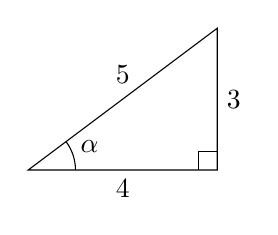
\begin{tikzpicture}[scale=0.6]
            % \draw (-4,0)--(0,0)--(0,3)--cycle; % Triangle with no labels
            \draw (-4,0)--(0,0) node[midway,below]{4}           % Side of length 4
                --(0,3) node[midway,right]{3}                   % Side of length 3
                --cycle node[midway,above=2pt]{5};              % Side of length 5
            \draw (-3,0) arc(0:{atan(3/4)}:1)                   % Arc denoting angle α
                node[midway,xshift=6pt,yshift=3pt]{$\alpha$};   % Label α
            \draw (-0.4,0)--(-0.4,0.4)--(0,0.4);
        \end{tikzpicture}
    \end{center}
    \end{minipage}
    \begin{minipage}{7cm}
    \begin{center}
        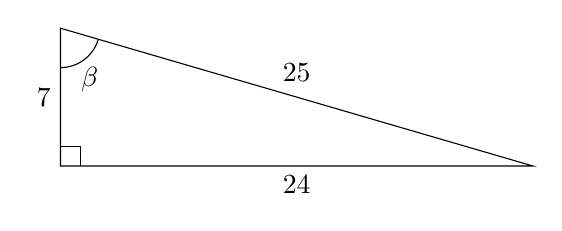
\begin{tikzpicture}[scale=0.25]
            % \draw (0,0)--(24,0)--(0,7)--cycle; % Triangle with no labels
            \draw (0,0)--(24,0) node[midway,below]{24}          % Side of length 24
                --(0,7) node[midway,above=2pt]{25}              % Side of length 25
                --cycle node[midway,left]{7};                   % Side of length 7
            \draw (0,5) arc(-90:{-atan(7/24)}:2)                % Arc denoting angle β
                node[midway,xshift=2pt,yshift=-7pt]{$\beta$};   % Label β
            \draw (1,0)--(1,1)--(0,1);
        \end{tikzpicture}
    \end{center}
    \end{minipage}
\end{center}
\vspace{-5pt} % Remove some of the vertical space created by \end{center}
Then $\beta=2\alpha$.
\end{corollary}
\begin{proof}
Exercise (use \Cref{double_angle}).
\end{proof}

You can generate other Pythagorean triples this way\footnote{In fact, you can generate \emph{all} Pythagorean triples this way. Can you figure out how?}.

\subsection{Other options}

There's no need to stick to the
\tcbox[colback=blue!10,colframe=blue,
    fontupper=\slshape,
    boxrule=1pt,boxsep=0pt,sharp corners,on line,
    top=2pt,bottom=2pt,left=2pt,right=2pt
]{status quo}
with \LaTeX\ formatting. You can go
\tcbox[blanker,fontupper=\sffamily\bfseries,
left=4mm,right=4mm,on line,
overlay={
    \draw[shift={([xshift=2mm]frame.west)},thin,red!70!black,fill=yellow] (0.05,0.3)--(-0.1,-0.1)--(0.02,-0.02)--(-0.05,-0.3)--(0.1,0.1)--(-0.02,0.02)--cycle;
    \draw[shift={([xshift=-2mm]frame.east)},thin,red!70!black,fill=yellow] (0.05,0.3)--(-0.1,-0.1)--(0.02,-0.02)--(-0.05,-0.3)--(0.1,0.1)--(-0.02,0.02)--cycle;}
]{WILD}
!

\begin{theorem}[colback=black,colframe=green,colupper=white,
    fontupper=\ttfamily,
    boxrule=4pt,
    interior style={left color=black,right color=black,middle color=gray!80!black}, % middle color must come AFTER left color and right color!
    frame style={top color=green,bottom color=orange,middle color=pink}, % middle color must come AFTER top color and bottom color!
    coltitle=red,boxed title style={colback=yellow,colframe=gray},
    ,overlay={
        \fill[pattern=horizontal lines,pattern color=red] ([xshift=-38mm]interior.south east)--++(8mm,0)--([yshift=30mm]interior.south east)--++(0,8mm)--cycle
        node[midway,shift={(0,-0.2*sqrt(2))},sloped,cyan,font=\sffamily\bfseries]{ENGINEERS LOVE THIS!};
    },
    breakable=false]{\normalfont\scshape Residue Theorem}{}
Suppose $\Omega$ is a simply connected open subset of $\C$, $\gamma$ is a positively oriented simple closed curve  in $\Omega$ and $f:\Omega\to\C$ is holomorphic on $\Omega$ except at the points $a_1,a_2,\ldots,a_n$ inside $\gamma$. Then:
\begin{center}
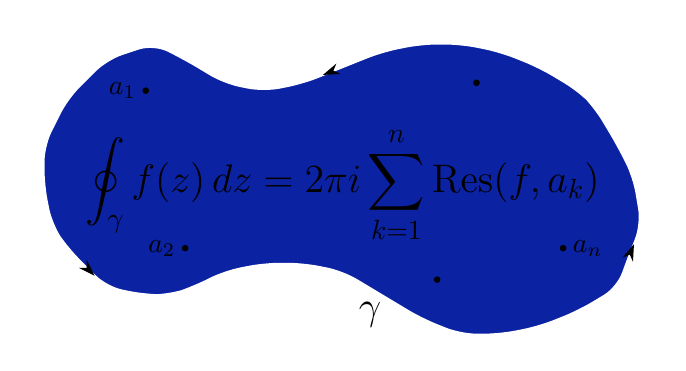
\begin{tikzpicture}[scale=1,every node/.style={transform shape}]
    \definecolor{col_int_gamma}{HTML}{0B22A3} % Color of Ω=int(γ)
    \clip (-4,-2) rectangle (4,2);
    \draw[-,thick,draw=white,rounded corners=2mm,fill=col_int_gamma] (0,-1.1)--(0.5,-1.4)--(1,-1.7)--(1.5,-1.9)--(2,-1.9)--(2.5,-1.8)--(3,-1.6)--(3.5,-1.3)--(3.6,-1)--(3.8,-0.5)--(3.7,0.1)--(3.5,0.5)--(3.2,1)--(3,1.2)--(2.5,1.5)--(2,1.7)--(1.5,1.8)--(1,1.8)--(0.5,1.7)--(0,1.5)--(-0.5,1.3)--(-1,1.2)--(-1.5,1.3)--(-2,1.6)--(-2.4,1.8)--(-2.7,1.7)--(-3,1.6)--(-3.5,1.1)--(-3.8,0.5)--(-3.8,0)--(-3.7,-0.5)--(-3.5,-0.8)--(-3.3,-1)--(-3,-1.3)--(-2.5,-1.4)--(-2.2,-1.4)--(-1.9,-1.3)--(-1.5,-1.1)--(-1,-1)--(-0.5,-1)--cycle;
    \draw[-{Stealth[length=6pt,width=4pt]}] (3.68,-0.8)--(3.7,-0.75);
    \draw[-{Stealth[length=6pt,width=4pt]}] (-0.2,1.42)--(-0.25,1.4);
    \draw[-{Stealth[length=6pt,width=4pt]}] (-3.21,-1.09)--(-3.15,-1.15);
    \fill (-2.5,1.2) circle (1.2pt) node[left]{$a_1$};
    \fill (-2,-0.8) circle (1.2pt) node[left]{$a_2$};
    \fill (1.2,-1.2) circle (1.2pt);
    \fill (2.8,-0.8) circle (1.2pt) node[right]{$a_n$};
    \fill (1.7,1.3) circle (1.2pt);
    \node[font=\Large] at (0.35,-1.65) {$\gamma$};
    \node[font=\Large] at (0,0) {$\displaystyle\oint_\gamma f(z)\,dz=2\pi i\sum_{k=1}^n \operatorname{Res}(f,a_k)$};
\end{tikzpicture}
\end{center}
\end{theorem}

A lot of nice integrals can be computed using the $\underbrace{\text{\href{http://residuetheorem.com/}{residue theorem}}}_{\textsf{Click on this link}}$, see \cite[\S5.2]{taylor}.\\
% \underbrace only works in math mode, so \text{...} is required to render text using it

\section{Macros}
\subsection{The \texttt{talign} environment}

The \verb!talign! and \verb!talign*! environments work like the \verb!align! and \verb!align*! environments, except they render equations in inline size. They have the same numbering and labeling options as \verb!align! and \verb!align*!.

\begin{verbbox}
\begin{align}
    \sum_{n=1}^2 \frac{1}{3n}=\int_0^1 x\,dx
\end{align}
\end{verbbox}

\begin{verbbox}
\begin{align*}
    \sum_{n=1}^2 \frac{1}{3n}=\int_0^1 x\,dx
\end{align*}
\end{verbbox}

\begin{verbbox}
\begin{talign}
    \sum_{n=1}^2 \frac{1}{3n}=\int_0^1 x\,dx
\end{talign}
\end{verbbox}

\begin{verbbox}
\begin{talign*}
    \sum_{n=1}^2 \frac{1}{3n}=\int_0^1 x\,dx
\end{talign*}
\end{verbbox}

\subsection{Vector and Matrix macros}

The \verb!\cvc!, \verb!\rvc! and \verb!\mat! commands can be used to typeset column vectors, row vectors and $m\times n$ matrices efficiently. The vector/matrix delimiters can also be changed, using the optional argument \texttt{p}, \texttt{b}, \texttt{B}, \texttt{v} or \texttt{V} (in accordance with \texttt{pmatrix}, \texttt{bmatrix}, \texttt{Bmatrix}, \texttt{vmatrix} or \texttt{Vmatrix} respectively from \href{https://ctan.org/pkg/amsmath}{\texttt{amsmath}}). The default is parentheses ( ). Of course, these commands can only be used in math mode.

\vspace{5pt}

\begin{multicols}{2}
\begin{verbbox}
$$\cvc{2,3,1}$$
\end{verbbox}

\begin{verbbox}
$$\rvc{5,7,6}$$
\end{verbbox}

\begin{verbbox}
$$\rvc{8,,4}$$
\end{verbbox}

\begin{verbbox}
$$\rvc{a,b_1,c^2,\&}$$
\end{verbbox}

\begin{verbbox}
$$\mat{4,8}{0,9}{6,3}$$
\end{verbbox}

\begin{verbbox}
$$\mat{1,7}{8,9,2,5}$$
\end{verbbox}
%%%%%%%%%%%%        %%%%%%%%%%%%        %%%%%%%%%%%%
\begin{verbbox}
$$\cvc[]{2,3,1}$$
\end{verbbox}

\begin{verbbox}
$$\rvc[p]{5,7,6}$$
\end{verbbox}

\begin{verbbox}
$$\rvc[b]{8,,4}$$
\end{verbbox}

\begin{verbbox}
$$\rvc[B]{a,b_1,c^2,\&}$$
\end{verbbox}

\begin{verbbox}
$$\mat[v]{4,8}{0,9}{6,3}$$
\end{verbbox}

\begin{verbbox}
$$\mat[V]{1,7}{8,9,2,5}$$
\end{verbbox}
\end{multicols}

\vspace{15pt}

{\sffamily From now on, every subsection will start on a new page (see the code for how to do this).}

\newcommand{\subsectionbreak}{\clearpage} % Start every subsection on a new page

\subsection{Box macros}

Here we provide three customizable \href{https://ctan.org/pkg/tcolorbox}{\texttt{tcolorbox}} environments that are perhaps less suited to theorem-type environments (but of course, they can still be used for these) and more suited to ``lower-level'' environments, e.g. discussions or examples one would like to explain in more detail.

\subsubsection*{The \texttt{filingbox} environment}

The \texttt{filingbox} environment is a \texttt{tcolorbox} environment that creates boxes in the shape of filing dividers. It has two optional arguments (the first delimited by parentheses, the second by brackets) and one mandatory argument.
\begin{itemize}
    \item The first optional argument specifies the position of the tab. It can be \texttt{ul} (up left), \texttt{uc} (up center), \texttt{ur} (up right), \texttt{dl} (down left), \texttt{dc} (down center) and \texttt{dr} (down right). The default is \texttt{ul}.
    \item The second optional argument specifies the color of the box. The background of the box is automatically set to this color with 10\% opacity. The default is black.
    \item The mandatory argument specifies the title.
\end{itemize}
Additional \texttt{tcolorbox} options can be specified after the title.

\begin{verbbox}
\begin{filingbox}{Title here}
This is a \textbf{filingbox}.
\end{filingbox}
\end{verbbox}

\begin{verbbox}
\begin{filingbox}(uc)[red]{Title here}
This is a \textbf{filingbox}.
\end{filingbox}
\end{verbbox}

\begin{verbbox}
\begin{filingbox}(ur){Title here}[halign=center]
This is a \textbf{filingbox}.
\end{filingbox}
\end{verbbox}

\begin{verbbox}
\begin{filingbox}(dl)[blue]{Title here}[left=20mm]
This is a \textbf{filingbox}.
\end{filingbox}
\end{verbbox}

\begin{verbbox}
\begin{filingbox}(dc){Title here}[before upper=\&]
This is a \textbf{filingbox}.
\end{filingbox}
\end{verbbox}

\begin{verbbox}
\begin{filingbox}(dr){Title here}[colupper=red]
This is a \textbf{filingbox}.
\end{filingbox}
\end{verbbox}

\subsubsection*{The \texttt{railingbox} environment}

The \texttt{railingbox} environment is a \texttt{tcolorbox} environment that creates boxes in the shape of railing bars. It is similar to the \texttt{filingbox} environment, except that it produces a box with sharp corners. It has the same argument structure as \texttt{filingbox}.

\begin{verbbox}
\begin{railingbox}{Title here}
This is a \textbf{railingbox}.
\end{railingbox}
\end{verbbox}

\begin{verbbox}
\begin{railingbox}(uc)[violet]{Title here}
This is a \textbf{railingbox}.
\end{railingbox}
\end{verbbox}

\begin{verbbox}
\begin{railingbox}(ur){Title here}[coltitle=orange]
This is a \textbf{railingbox}.
\end{railingbox}
\end{verbbox}

\begin{verbbox}
\begin{railingbox}(dl)[teal]{Title here}
This is a \textbf{railingbox}.
\end{railingbox}
\end{verbbox}

\begin{verbbox}
\begin{railingbox}(dc){Title here}[after upper=DC]
This is a \textbf{railingbox}.
\end{railingbox}
\end{verbbox}

\begin{verbbox}
\begin{railingbox}(dr)[pink]{Title here}
This is a \textbf{railingbox}.
\end{railingbox}
\end{verbbox}

\subsubsection*{The \texttt{flagbox} environment}

The \texttt{flagbox} environment is a \texttt{tcolorbox} environment that creates boxes in the shape of flags. It has the same argument structure as \texttt{filingbox}, except that the position of the tab can only be \texttt{ul}, \texttt{ur}, \texttt{dl} or \texttt{dr} (the default is still \texttt{ul}).

\begin{verbbox}
\begin{flagbox}{Title here}
This is a \textbf{flagbox}.\\

The flagpole extends to the bottom of the box.
\end{flagbox}
\end{verbbox}
\begin{verbbox}
\begin{flagbox}(ur)[orange]{Title here}
This is a \textbf{flagbox}.\\

The flagpole extends to the bottom of the box.
\end{flagbox}
\end{verbbox}
\begin{verbbox}
\begin{flagbox}(dl)[purple]{Title here}
This is a \textbf{flagbox}.\\

The flagpole extends to the top of the box.
\end{flagbox}
\end{verbbox}
\begin{verbbox}
\begin{flagbox}(dr){Title here}[fontupper=\itshape]
This is a \textbf{flagbox}.\\

The flagpole extends to the top of the box.
\end{flagbox}
\end{verbbox}

\subsection{Ball macros}

The command \verb!\solidball! produces a customizable solid pool ball. It has four arguments, two optional and two mandatory.
\begin{itemize}
    \item The first (optional) argument specifies the text in the center of the ball. The default is blank (no text). The text format can also be manually specified, e.g. with \verb!\color{white} abc!.
    \item The second (mandatory) argument specifies the color of the ball.
    \item The third (optional) argument specifies the color of the ``background'' of the ball, i.e. the area behind the text (though it will be shown even if there is no text). The default is \texttt{white}.
    \item The fourth (mandatory) argument specifies the size of the ball. If this is \texttt{1}, the diameter of the ball will be 1 cm. This argument can be specified as an integer (e.g. \texttt{2}), a floating-point number (e.g. \texttt{0.75}) or a mathematical expression (e.g. \texttt{2*3/8}).
\end{itemize}

There is also a starred version \verb!\solidball*!, where the background is not drawn. In this version, the third argument is redundant.

\begin{tcolorbox}[blanker,sidebyside,before skip=10pt,after skip=10pt]
\begin{verbbox}[righthand width=1.3cm]
\solidball{red}{1}
\end{verbbox}
\begin{verbbox}[righthand width=1.3cm]
\solidball[2]{blue}{0.8}
\end{verbbox}
\begin{verbbox}[righthand width=1.3cm]
\solidball{green}[pink]{0.6}
\end{verbbox}
\begin{verbbox}[righthand width=1.3cm]
\solidball[3a]{violet}[red]{1}
\end{verbbox}
\tcblower %%%%%%%% %%%%%%%% %%%%%%%% %%%%%%%%
\begin{verbbox}[righthand width=1.3cm]
\solidball*{red}{1}
\end{verbbox}
\begin{verbbox}[righthand width=1.3cm]
\solidball*[\$]{yellow}{4/5}
\end{verbbox}
\begin{verbbox}[righthand width=1.3cm]
\solidball*{blue}[green]{(9-3)/10}
\end{verbbox}
\begin{verbbox}[righthand width=1.3cm]
\solidball*[6Z]{gray}[blabla]{1}
\end{verbbox}
\end{tcolorbox}

The command \verb!\stripedball! produces a customizable striped pool ball. It has the same argument structure as \verb!\solidball!, as well as a starred version that omits the background (but the stripe is still drawn, so the third argument is no longer redundant).

\begin{tcolorbox}[blanker,sidebyside,before skip=10pt,after skip=10pt]
\begin{verbbox}[righthand width=1.3cm]
\stripedball{yellow}{1}
\end{verbbox}
\begin{verbbox}[righthand width=1.3cm]
\stripedball[2]{violet}{0.5}
\end{verbbox}
\begin{verbbox}[righthand width=1.3cm]
\stripedball{orange}[blue]{.75}
\end{verbbox}
\begin{verbbox}[righthand width=1.3cm]
\stripedball[$\rho$]{red}[green]{1}
\end{verbbox}
\tcblower %%%%%%%% %%%%%%%% %%%%%%%% %%%%%%%%
\begin{verbbox}[righthand width=1.3cm]
\stripedball*{green}{1}
\end{verbbox}
\begin{verbbox}[righthand width=1.3cm]
\stripedball*[V]{white}[brown]{1/2}
\end{verbbox}
\begin{verbbox}[righthand width=1.3cm]
\stripedball*{black}{sqrt(9/16)}
\end{verbbox}
\begin{verbbox}[righthand width=1.3cm]
\stripedball*[mb]{pink}[yellow]{1}
\end{verbbox}
\end{tcolorbox}

\newpage % Page break, i.e. skip to the next page

The command \verb!\poolball! is based on \verb!\solidball! and \verb!\stripedball! and produces the standard (Aramith Tournament) pool balls. It has one optional argument and two mandatory arguments.
\begin{itemize}
    \item The optional argument specifies the text in the center of the ball. If this is not specified, the value of the first mandatory argument will be used.
    \item The first mandatory argument specifies the number on the ball (the color and whether it is solid or striped are automatically determined from this). If this is \texttt{0} (or any multiple of 16), it will produce the cue ball.
    \item The second mandatory argument specifies the size of the ball (identically to \verb!\solidball! and \verb!\stripedball!).
\end{itemize}

\begin{center}
\renewcommand*{\arraystretch}{1.25} % Redefine \arraystretch for this table only
\begin{tabular}{cccc}
    \poolball{1}{1} & \poolball{2}{1} & \poolball{3}{1} & \poolball{4}{1} \\
    \verb!\poolball{17}{1}! & \verb!\poolball{2}{1}! & \verb!\poolball{3}{1}! & \verb!\poolball{4}{1}! \\[4pt]
    \poolball{5}{1} & \poolball{6}{1} & \poolball{7}{1} & \poolball{8}{1} \\
    \verb!\poolball{5}{1}! & \verb!\poolball{6}{1}! & \verb!\poolball{7}{1}! & \verb!\poolball{8}{1}! \\[4pt]
    \poolball{9}{1} & \poolball{10}{1} & \poolball{11}{1} & \poolball{12}{1} \\
    \verb!\poolball{9}{1}! & \verb!\poolball{10}{1}! & \verb!\poolball{11}{1}! & \verb!\poolball{12}{1}! \\[4pt]
    \poolball{13}{1} & \poolball{14}{1} & \poolball{15}{1} & \poolball{0}{1} \\
    \verb!\poolball{13}{1}! & \verb!\poolball{14}{1}! & \verb!\poolball{15}{1}! & \verb!\poolball{0}{1}!
\end{tabular}
\end{center}

The first argument is only defined modulo 16, so \verb!\poolball{19}{1}! and \verb!\poolball{-13}{1}! produce the same result as \verb!\poolball{3}{1}!.

\subsection{Smart Operator Macros}

The \verb!\Sum! command is a ``smart'' version of the \verb!\sum! command (provided by \LaTeX) that incorporates styles and upper and lower limits into its arguments. It is based on the options provided by \href{https://ctan.org/pkg/amsmath}{\texttt{amsmath}}.\\

The \verb!\Sum! command takes one optional argument and one set of mandatory arguments, separated by commas.

\begin{itemize}
\newcommand{\argnumber}[1]{ % This command is only defined locally, i.e. only within the itemize list
    \ifnum#1=1\texttt{\color{red!80!black}\#1}\fi
    \ifnum#1=2\texttt{\color{Orange!80!black}\#2}\fi
    \ifnum#1=3\texttt{\color{Dandelion!80!black}\#3}\fi
    \ifnum#1=4\texttt{\color{Green!80!black}\#4}\fi
    \ifnum#1=5\texttt{\color{blue!80!black}\#5}\fi
}
    \item If no mandatory argument is present, the sum is over $n$ and runs from $n=1$ to $\infty$.
    \item If one mandatory argument \argnumber{1} is present, the sum is over $n$ and runs from $n=$\argnumber{1} to $\infty$.
    \item If two mandatory arguments \argnumber{1},\argnumber{2} are present, the sum is over $n$ and runs from $n=$\argnumber{1} to \argnumber{2}.
    \item If three mandatory arguments \argnumber{1},\argnumber{2},\argnumber{3} are present, the sum is over \argnumber{1} and runs from \argnumber{1} =\argnumber{2} to \argnumber{3}.
    \item If four mandatory arguments \argnumber{1},\argnumber{2},\argnumber{3},\argnumber{4} are present, the sum is over \argnumber{1} \emph{and} \argnumber{2} and runs from \argnumber{1},\argnumber{2} =\argnumber{3} to \argnumber{4}.
    \item If five mandatory arguments \argnumber{1},\argnumber{2},\argnumber{3},\argnumber{4},\argnumber{5} are present, the sum is over \argnumber{1},\argnumber{2} \emph{and} \argnumber{3} runs from \argnumber{1},\argnumber{2},\argnumber{3} =\argnumber{4} to \argnumber{5}.
\end{itemize}
\begin{warning}
    The mandatory argument cannot be omitted! Simply writing \verb!\Sum! will lead to errors.
\end{warning}

\subsubsection*{Inline mode}

\begin{multicols}{2} % Inline versions
\tcbset{height=0.8cm} % Locally fix tcolorbox height to match boxes next to each other
\begin{verbbox}
$\Sum{}$
\end{verbbox}

\begin{verbbox}
$\Sum{3,8}$
\end{verbbox}

\begin{verbbox}
$\Sum{i,j,\Omega,\tau}$
\end{verbbox}
%%%%%%%%%%%%        %%%%%%%%%%%%        %%%%%%%%%%%%
\begin{verbbox}
$\Sum{4}$
\end{verbbox}

\begin{verbbox}
$\Sum{m,6,25}$
\end{verbbox}

\begin{verbbox}
$\Sum{\&,\$,\{,?,+}$
\end{verbbox}
\end{multicols}

\subsubsection*{Display mode}

\begin{multicols}{2} % Display versions
\tcbset{height=1.5cm} % Locally fix tcolorbox height to match boxes next to each other
\begin{verbbox}
$$\Sum{}$$
\end{verbbox}

\begin{verbbox}
$$\Sum{3,8}$$
\end{verbbox}

\begin{verbbox}
$$\Sum{i,j,\Omega,\tau}$$
\end{verbbox}
%%%%%%%%%%%%        %%%%%%%%%%%%        %%%%%%%%%%%%
\begin{verbbox}
$$\Sum{4}$$
\end{verbbox}

\begin{verbbox}
$$\Sum{m,6,25}$$
\end{verbbox}

\begin{verbbox}
$$\Sum{\&,\$,\{,?,+}$$
\end{verbbox}
\end{multicols}

The optional argument of the \verb!\Sum! command specifies the style of the sum. The standard \verb!\sum! command can be customized in the following ways:
\begin{itemize}
    \item By adding \verb!\limits! (to show the limits above and below the sum) or \verb!\nolimits! (to show the limits beside the sum). These are added \emph{after} the command \verb!\sum!.
    \item It can also be customized by adding \verb!\textstyle! (to show the sum in inline style) or \verb!\displaystyle! (to show the sum in display style). These are added \emph{before} the command \verb!\sum!.
\end{itemize}
In the smart \verb!\Sum! command, these options are incorporated into the optional argument.\\

There are eight options for the optional argument of \verb!\Sum!:
\vspace*{-10pt}
\begin{multicols}{2}
\begin{itemize}[leftmargin=0.5in,labelsep=0.3in]
    \item[\texttt{l}] Limits above and below
    \item[\texttt{n}] Limits beside
    \item[\texttt{i}] Inline style
    \item[\texttt{d}] Display style
    \item[\texttt{il}] Inline style with limits above and below
    \item[\texttt{in}] Inline style with limits beside
    \item[\texttt{dl}] Display style with limits above and below
    \item[\texttt{dn}] Display style with limits beside
\end{itemize}
\end{multicols}

The optional argument overrides any pre-defined options, i.e. \verb!\textstyle\Sum[d]{8}! is equivalent to \verb!\Sum[d]{8}!.\\

If the optional argument is empty, it will be treated as absent, i.e. \verb!\Sum[]{8}! is equivalent to \verb!\Sum{8}!.

\begin{multicols}{2}
\tcbset{height=1.5cm} % Locally fix tcolorbox height to match boxes next to each other
\begin{verbbox}
$$\Sum[l]{}$$
\end{verbbox}

\begin{verbbox}
$$\Sum[n]{}$$
\end{verbbox}

\begin{verbbox}
$$\Sum[i]{}$$
\end{verbbox}

\begin{verbbox}
$$\Sum[d]{}$$
\end{verbbox}
%%%%%%%%%%%%        %%%%%%%%%%%%        %%%%%%%%%%%%
\begin{verbbox}
$$\Sum[il]{}$$
\end{verbbox}

\begin{verbbox}
$$\Sum[in]{}$$
\end{verbbox}

\begin{verbbox}
$$\Sum[dl]{}$$
\end{verbbox}

\begin{verbbox}
$$\Sum[dn]{}$$
\end{verbbox}
\end{multicols}

All of the standard large operators have a ``smart'' version, as shown below:

\begin{center}
\renewcommand*{\arraystretch}{1.5} % Redefine \arraystretch for this table only
\begin{tabular}{ccccccc}
    Standard operator & \verb!\sum! & \verb!\prod! & \verb!\coprod! & \verb!\bigcap! & \verb!\bigcup! & \verb!\bigsqcup! \\
    Smart operator & \verb!\Sum! & \verb!\Prod! & \verb!\Coprod! & \verb!\Capp! & \verb!\Cupp! & \verb!\Kupp! \\
    Inline style & $\Sum[i]{}$ & $\Prod[i]{}$ & $\Coprod[i]{}$ & $\Capp[i]{}$ & $\Cupp[i]{}$ & $\Kupp[i]{}$ \\
    Display style & $\Sum[d]{}$ & $\Prod[d]{}$ & $\Coprod[d]{}$ & $\Capp[d]{}$ & $\Cupp[d]{}$ & $\Kupp[d]{}$ \\[12pt] % Add extra vertical space here
    Standard operator & \verb!\bigodot! & \verb!\bigoplus! & \verb!\bigotimes! & \verb!\biguplus! & \verb!\bigwedge! & \verb!\bigvee! \\
    Smart operator & \verb!\Odot! & \verb!\Oplus! & \verb!\Otimes! & \verb!\Uplus! & \verb!\Wedge! & \verb!\Vee! \\
    Inline style & $\Odot[i]{}$ & $\Oplus[i]{}$ & $\Otimes[i]{}$ & $\Uplus[i]{}$ & $\Wedge[i]{}$ & $\Vee[i]{}$ \\
    Display style & $\Odot[d]{}$ & $\Oplus[d]{}$ & $\Otimes[d]{}$ & $\Uplus[d]{}$ & $\Wedge[d]{}$ & $\Vee[d]{}$
\end{tabular}
\end{center}

However, if you want something more elaborate, such as $\Disp\sum_{n\in\Z\exc\{0\}}$, it is easier to type it out normally.\\

To create your own smart operator, add the following lines (for example) to the preamble:

\begin{verbatim}
        \DeclareMathOperator*{\TheOp}{Sym}
        \CreateSmartLargeOperator{TheOp}{SmartOp}
\end{verbatim}

Then the command \verb!\SmartOp{2}! will produce $\operatorname*{Sym}_{n=2}^\infty$ in inline mode and $\Disp\operatorname*{Sym}_{n=2}^\infty$ in display mode.\\

The first line defines \verb!\TheOp! as the operator denoted by Sym. The second line defines \verb!\SmartOp! as the smart version of this operator. Note that neither argument in the second line has a backslash, this is important. And of course, the operator only renders in math mode.

\subsection{Miscellaneous}

Some commands have been defined to convenience typing in \LaTeX. For example, the symbol $\R$ for real numbers is normally typed as \verb!\mathbb{R}!, which is rather cumbersome.

\begin{center}
    \begin{tabular}{*{5}{c}} % *{5}{c} is a shortcut for ccccc
        $\A$ & $\As$ & $\Abar$ & $\Ab$ & $\Atil$ \\
        \verb!\A! & \verb!\As! & \verb!\Abar! & \verb!\Ab! & \verb!\Atil!
    \end{tabular}
\end{center}

The above commands have been defined similarly for all letters of the alphabet, with exceptions for pre-defined commands (e.g. \verb!\S!, which renders as \S).\\

The \href{https://ctan.org/pkg/physics}{\texttt{physics}} package defines bracket-like commands (such as \verb!\abs! and \verb!\norm!) that automatically resize themselves according to their content. Here, we have defined the commands \verb!\floor! and \verb!\ceil! with the same features.

\begin{multicols}{2}
\begin{verbbox}[righthand width=3cm]
$\floor{4.1}$
\end{verbbox}
\begin{verbbox}[righthand width=3cm]
$\floor{x^2}$
\end{verbbox}
\begin{verbbox}[righthand width=3cm]
$\floor{\dfrac{9}{5}}$
\end{verbbox}
\begin{verbbox}[righthand width=3cm]
$\floor*{\dfrac{x^4}{y^7}}$
\end{verbbox}
%%%%%%%%%%%% %%%%%%%%%%%% %%%%%%%%%%%%
\begin{verbbox}[righthand width=3cm]
$\ceil{7.6}$
\end{verbbox}
\begin{verbbox}[righthand width=3cm]
$\ceil{x^5}$
\end{verbbox}
\begin{verbbox}[righthand width=3cm]
$\ceil{\dfrac{3}{7}}$
\end{verbbox}
\begin{verbbox}[righthand width=3cm]
$\ceil*{\dfrac{x^5}{y^3}}$
\end{verbbox}
\end{multicols}

The starred versions \verb!\floor*! and \verb!\ceil*! do not resize the brackets.\\

The \texttt{physics} package also defines the identical commands \verb!\ip! and \verb!\braket! for inner products. Here, we have redefined \verb!\ip! to take only one argument (which may contain commas), while \verb!\braket! is left as it is. Both commands have automatic resizing, which is suppressed with their starred versions.

\begin{multicols}{2}
\begin{verbbox}
$\ip{x,y}$
\end{verbbox}
%%%%%%%%%%%% %%%%%%%%%%%% %%%%%%%%%%%%
\begin{verbbox}
$\braket{x}{y}$
\end{verbbox}
\end{multicols}

The \href{https://ctan.org/pkg/amsmath}{\texttt{amsmath}} package provides various macros for trigonometric functions, such as $\verb!\sin!$ for sin. The \texttt{physics} package overwrites these macros and provides additional ones, all with automatic resizing of brackets (unless the package is loaded with the option \texttt{notrig}). Here we have extended this list of macros to the following (all with automatic resizing):

\begin{center}
    \begin{tabular}{*{9}{c}} % *{9}{c} is a shortcut for ccccccccc
        sin & asin & arcsin & sinh & asinh & arsinh & arcsinh & sen  & Re \\
        cos & acos & arccos & cosh & acosh & arcosh & arccosh & tg   & Im \\
        tan & atan & arctan & tanh & atanh & artanh & arctanh & ctg  & arg \\
        cot & acot & arccot & coth & acoth & arcoth & arccoth & senh & Arg \\
        sec & asec & arcsec & sech & asech & arsech & arcsech & tgh  & im \\
        csc & acsc & arccsc & csch & acsch & arcsch & arccsch & ctgh & ker
    \end{tabular}
\end{center}

\LaTeX\ provides a command \verb!\iff! which renders as $\Longleftrightarrow$ (identical to \verb!\Longleftrightarrow!). The \texttt{amsmath} package also provides two commands, \verb!\implies! which renders as $\Longrightarrow$ (identical to \verb!\Longrightarrow!), and \verb!\impliedby! which renders as $\Longleftarrow$ (identical to \verb!\Longleftarrow!).\\

Here, these three commands are redefined to produce shorter sets of arrows, $\Leftrightarrow$, $\Rightarrow$ and $\Leftarrow$, identical to \verb!\Leftrightarrow!, \verb!\Rightarrow! and \verb!\Leftarrow! respectively. The original (long) arrows can be obtained using the starred versions \verb!\iff*!, \verb!\implies*! and \verb!\impliedby*!.\\

Unlike the original commands, these can also be used in text mode, however the spacing needs to be accounted for depending on the text/math on either side of the arrows.

\begin{verbbox}
a\iff b\implies c\impliedby d
\end{verbbox}

\begin{verbbox}
a\iff* b\implies* c\impliedby* d
\end{verbbox}

\begin{verbbox}
$a\iff b\implies c\impliedby d$
\end{verbbox}

\begin{verbbox}
$a\iff* b\implies* c\impliedby* d$
\end{verbbox}

\newpage
\phantomsection % Required if hyperref is used
\addcontentsline{toc}{section}{References} % Adding bibliography to table of contents
\printbibliography % Print the bibliography

\vspace{10pt}

If you're struggling to find the \LaTeX\ command for a symbol, go to \Href{https://detexify.kirelabs.org/}{detexify.kirelabs.org}.\\

If you're looking for ideas/inspiration for your \LaTeX\ documents, check out these websites:
\begin{itemize}[leftmargin=0.5in]
    \item \Href{https://castel.dev/}{castel.dev}
    \item \Href{http://dec41.user.srcf.net/}{dec41.user.srcf.net}
    \item \Href{https://www.youtube.com/@DrTrefor}{youtube.com/@DrTrefor}
    \item \Href{https://coffeeintotheorems.com/}{coffeeintotheorems.com}
    \item \Href{https://www.physicsread.com/}{physicsread.com}
    \item \Href{https://www.latextemplates.com/}{latextemplates.com}
    \item \Href{https://ralphs16.github.io/}{ralphs16.github.io}
    \item \Href{https://github.com/vhbelvadi/}{github.com/vhbelvadi}
\end{itemize}

As well as \Href{https://tex.stackexchange.com/}{tex.stackexchange.com} and \Href{https://stackoverflow.com/}{stackoverflow.com}, where you can ask and answer questions.\\

And of course, the Overleaf gallery: \Href{https://www.overleaf.com/latex/templates/}{overleaf.com/latex/templates}.\\

\centering Have fun! \coolqed{0.32}

\end{document}